\documentclass[aps,prapplied,twocolumn,superscriptaddress,floatfix,longbibliography]{revtex4-2}
\usepackage{amsmath,amssymb,amsfonts}
\usepackage{graphicx}
\usepackage{bm}
\usepackage{tikz}
\usepackage[american]{circuitikz}
\usepackage[colorlinks=true,linkcolor=blue,citecolor=blue,urlcolor=blue]{hyperref}
\usetikzlibrary{patterns,arrows.meta}

\begin{document}

\title{Metric loading: An exactly solvable stability threshold for non-Foster transmission-line metamaterials}

\author{Dino \v{S}krgi\'c}
\email{dinoskrg@buffalo.edu}
\affiliation{Department of Physics, University at Buffalo, State University of New York, Buffalo, NY 14260, USA}
\author{Dado \v{S}krgi\'c}
\email{dado.skrgic@fer.hr}
\affiliation{Faculty of Electrical Engineering and Computing, University of Zagreb, 10000 Zagreb, Croatia}
\author{Dejan Stojkovic}
\email{ds77@buffalo.edu}
\affiliation{Department of Physics, University at Buffalo, State University of New York, Buffalo, NY 14260, USA}

\date{\today}

\begin{abstract}
Non-Foster elements promise transmission-line metamaterials free of the bandwidth limits of Foster's reactance theorem, but their use is held back by instability, for which existing criteria are applied network by network. We study a two-dimensional transmission-line strip loaded by rows of shunt capacitors and show that the capacitance profile acts as an energy metric: the sign of a mode's stored energy equals the sign of its capacitance-weighted norm. In any lossless network of positive inductors, the number of non-oscillatory growing modes equals the number of negative eigenvalues of the nodal capacitance matrix, so no width, length, or termination stabilizes ordinary negative capacitors. When each negative shunt capacitor is paired with a velocity-matched negative series inductance along its row, the negative-energy modes are lifted above zero frequency by transverse confinement. For rows of alternating sign this gives a closed-form threshold on the transverse wavenumber, a maximum width for a grounded strip, and the counterintuitive result that stronger negative loading is more stable. At nominal matching the tolerance to element errors is below 1\%, but biasing the passive rows toward over-matching and the active rows toward under-matching widens it to about $\pm10\%$ in the series inductors. Above threshold the strip still carries negative-energy modes at real frequency, and dissipation makes them grow at a few times $\omega/Q$. The threshold therefore separates latch-up from loss-driven oscillation, and full stability requires the negative-impedance converters to supply a net gain between about 0.8 and 1.4 times the passive loss.
\end{abstract}

\maketitle

\section{Introduction}

Periodically loaded transmission lines are the workhorse of microwave metamaterials~\cite{Eleftheriades_2002:TMTT,Caloz_2006:book}. The capacitively loaded line is textbook material~\cite{Pozar_2012:book}, and the band-structure ideas behind it are those of photonic crystals~\cite{Joannopoulos_2008:book}. Passive loading is stable but band-limited by Foster's reactance theorem~\cite{Foster_1924:BSTJ}. Non-Foster elements, that is, negative capacitors and inductors synthesized with negative-impedance converters (NICs)~\cite{Linvill_1953:PIRE}, were proposed to lift this limit~\cite{Tretyakov_2001:MOTL}. They have since been used for broadband matching of small antennas~\cite{SussmanFort_2009:TAP}, for superluminal and nearly dispersionless lines~\cite{Sievenpiper_2011:AWPL,Hrabar_2011:APL,Long_2014:TMTT,Long_2018:TMTT}, and in a range of active metamaterials~\cite{Hrabar_2018:EPJAM}.

The price is stability. An NIC relies on positive feedback, and a network that contains non-Foster elements can self-oscillate or latch up. In his review of the first decade of active metamaterials, Hrabar identifies stability management as the main obstacle to their wider use and notes that it is still not well understood~\cite{Hrabar_2018:EPJAM}. Rigorous tools exist, among them Laplace-domain pole analysis~\cite{Hrabar_2012:Automatika,Loncar_2017:TAP}, the normalized determinant function~\cite{Tang_2017:TMTT}, circuit-level stability and bifurcation analysis~\cite{Suarez_2018:TMTT}, and stability theory formulated for non-Foster circuits and elements~\cite{Stearns_2011:APS,Stearns_2013:IMS,Ugarte_2012:TAP}. They are applied network by network, however, and several observations have resisted a unified explanation. The widely used rule that the total capacitance must remain positive has counterexamples, the simplest being an ideal positive and an ideal negative capacitor joined by a transmission line of any nonzero length, which is always unstable~\cite{Loncar_2017:TAP}. Periodically loaded lines that are stable for a few cells can become unstable for many~\cite{Rengarajan_2013:AWPL}. Element dispersion matters as well, since band-limited negative capacitors are stable over a wider range of loads than ideal ones~\cite{Zanic_2024:AIPA}. Two-dimensional structures, the natural setting for metamaterials, have received the least attention; their stability has been studied mainly by applying the Nyquist criterion to equivalent circuits~\cite{Rajab_2010:JAP}. What has been missing is a distributed non-Foster structure whose stability boundary can be written in closed form, so that the mechanism can be read off directly.

This paper provides such a structure, a two-dimensional (2D) transmission-line strip loaded by rows of lumped elements. Shunt loads change the capacitance profile of the medium, and the capacitance profile weighs the stored electric energy. It therefore acts as a metric, in the sense that the sign of a mode's capacitance-weighted norm is the sign of its stored energy. Negative capacitors create modes of negative stored energy, and stability becomes a kinematic question of whether such a mode can be pulled down to zero frequency. In the theory of Hamiltonian systems the sign of a mode's energy is its Krein signature, and its consequences, namely negative-energy waves, collisions between modes of opposite signature, and absolute instability, are well developed~\cite{Kapitula_2013:book,Kollar_2014:SIREV,Cairns_1979:JFM,Briggs_1964:book}. We use that language sparingly, and Table~\ref{tab:dictionary} translates each term into circuit language.

For ideal lossless elements the analysis is exact. In any lossless network of positive inductors, Sylvester's law of inertia fixes the number of exponentially growing, non-oscillating modes at the number of negative eigenvalues of the nodal capacitance matrix. The positive-total-capacitance rule is the one-node case of this count, the counterexample of Ref.~\cite{Loncar_2017:TAP} follows at once, and no geometry can stabilize ordinary negative capacitors. When each negative shunt capacitor is instead paired with a negative series inductance along its row, chosen so that the row keeps the host phase velocity, the negative-energy modes are lifted by transverse confinement. For rows of alternating sign the strip is then stable if and only if its transverse wavenumber exceeds a threshold $\chi_*$ set by a single transcendental equation, which translates into a maximum width for a grounded strip. The matching between shunt and series elements fixes an asymmetric tolerance window that can be widened by design. Losses do not move the threshold but change its meaning, because the negative-energy modes that survive above it are driven unstable by dissipation, and stability then requires the NICs to supply a controlled net gain.

The structure was first conceived as a circuit analogue of multi-brane models of gravity~\cite{Dvali_2000:PLB,Dai_2014:PRD}, in which $r_0$ below plays the role of a crossover length. Nothing in this paper depends on that origin.

\begin{table}[t]
\caption{Physics terms used in the stability literature and their circuit meaning in this paper.}
\label{tab:dictionary}
\begin{ruledtabular}
\begin{tabular}{p{0.34\columnwidth}p{0.58\columnwidth}}
Physics term & Circuit meaning \\ \hline
Metric $W(y)$ & Capacitance profile, normalized to the host \\
Krein signature & Sign of a mode's stored energy, $\operatorname{sign}\langle\phi,W\phi\rangle$ \\
Negative-energy mode & Mode whose excitation lowers the total stored energy; bound to the negative rows \\
Operator $-\partial_y^2$ & Magnetic energy of the host along $y$ \\
Krein collision at $\omega=0$ & Negative-energy mode pulled to dc; real right-half-plane pole $s=+\sigma$ (latch-up without oscillation) \\
Krein collision at $\omega\neq0$ & Two modes of opposite energy meet at finite frequency; complex right-half-plane pole pair (oscillation) \\
Absolute instability & Growth in place at zero group velocity; not removed by matched terminations or finite length \\
Matched loading & Velocity-matched row, $L_LC_L=L_0C_0$ \\
Transverse wavenumber $k_x$ & Transverse resonance of the grounded strip; cutoff $v_pk_x/2\pi$ \\
\end{tabular}
\end{ruledtabular}
\end{table}

\section{The loaded strip and its energy metric}
\label{sec:model}

\begin{figure}[t]
\centering
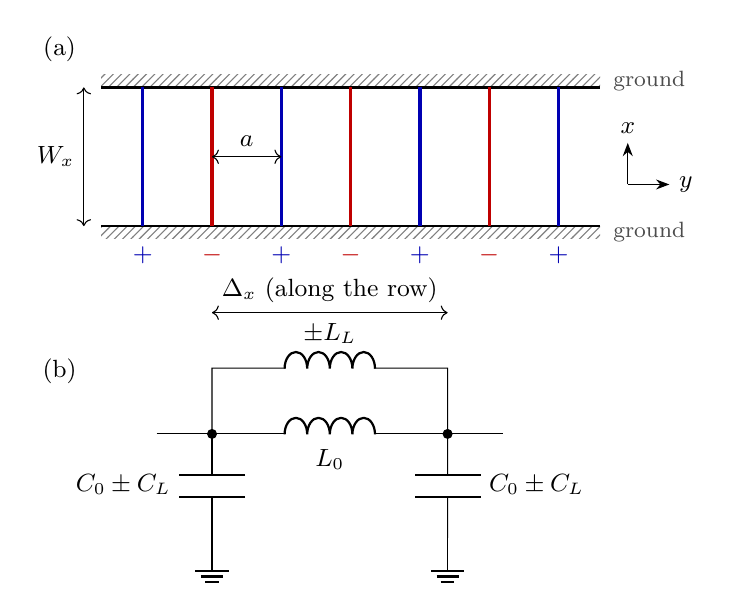
\begin{tikzpicture}[scale=0.88, every node/.style={font=\small}]
  \node at (-0.6,2.55) {(a)};
  \fill[pattern=north east lines, pattern color=gray] (0,2.0) rectangle (7.2,2.18);
  \fill[pattern=north east lines, pattern color=gray] (0,-0.18) rectangle (7.2,0.0);
  \draw[thick] (0,0) -- (7.2,0); \draw[thick] (0,2) -- (7.2,2);
  \foreach \i in {0,...,6} {
    \pgfmathsetmacro{\yy}{0.6+\i*1.0}
    \ifodd\i
      \draw[very thick, red!75!black] (\yy,0) -- (\yy,2);
      \node[red!75!black] at (\yy,-0.42) {$-$};
    \else
      \draw[very thick, blue!70!black] (\yy,0) -- (\yy,2);
      \node[blue!70!black] at (\yy,-0.42) {$+$};
    \fi
  }
  \draw[<->] (1.6,1.0) -- node[above]{$a$} (2.6,1.0);
  \draw[<->] (-0.25,0) -- node[left]{$W_x$} (-0.25,2);
  \node[gray!60!black, right] at (7.25,2.09) {\footnotesize ground};
  \node[gray!60!black, right] at (7.25,-0.09) {\footnotesize ground};
  \draw[-{Stealth}] (7.6,0.6) -- (8.2,0.6) node[right]{$y$};
  \draw[-{Stealth}] (7.6,0.6) -- (7.6,1.2) node[above]{$x$};
  \begin{scope}[shift={(1.6,-3.0)}]
    \node at (-2.2,0.9) {(b)};
    \draw (0,0) to[L, l_=$L_0$, *-*] (3.4,0);
    \draw (0,0) -- (0,0.95) to[L, l=$\pm L_L$] (3.4,0.95) -- (3.4,0);
    \draw (0,0) to[C, l_=$C_0\pm C_L$] (0,-1.5) node[ground]{};
    \draw (3.4,0) to[C, l=$C_0\pm C_L$] (3.4,-1.5) node[ground]{};
    \draw (-0.8,0) -- (0,0); \draw (3.4,0) -- (4.2,0);
    \draw[<->] (0,1.75) -- node[above]{$\Delta_x$ (along the row)} (3.4,1.75);
  \end{scope}
\end{tikzpicture}
\caption{(a) Top view of a grounded strip of width $W_x$. The loaded rows (colored lines) run along $x$, are stacked along $y$ with spacing $a$, and alternate between positive loading ($+$, ordinary elements) and negative loading ($-$, non-Foster elements); the hatched lines are the grounded edges. (b) One cell of a loaded row, of pitch $\Delta_x$ along the row. Each row node carries a shunt capacitor $\pm C_L$ in parallel with the host node capacitance $C_0$, and each link along the row carries an inductor $\pm L_L$ in parallel with the host link inductance $L_0$. On negative rows both added elements are realized with NICs. Matched loading, $L_LC_L=L_0C_0=(\Delta_x/v_p)^2$, keeps the phase velocity of a loaded row equal to the host phase velocity $v_p$. Whenever $C_L>C_0$, as in all designs of Table~\ref{tab:hardware} except the 0.5-pF one, $L_L<L_0$ and the net link inductance of a negative row, the parallel combination of $L_0$ and $-L_L$, is itself negative.}
\label{fig:schematic}
\end{figure}

The host is a uniform, isotropic 2D transmission-line medium with phase velocity $v_p$, in the sense of the planar metamaterial media of Ref.~\cite{Eleftheriades_2002:TMTT}: an array of parallel lanes along $y$, each a line with per-unit-length capacitance $C'$ and inductance $L'$, joined to its neighbors by series inductance along $x$. The lanes have pitch $\Delta_x$, so $v_p=1/\sqrt{L'C'}$ and, per cell of length $\Delta_x$, the host has node capacitance $C_0=C'\Delta_x$ and link inductance $L_0=L'\Delta_x$. In a printed realization the coupling along $y$ is also discretized, and the continuum along $y$ used below is the limit in which that discretization is fine compared with the row spacing $a$ and the length $r_0$ defined below. Rows of lumped elements are placed at $y=na$, as shown in Fig.~\ref{fig:schematic}. Each row node carries a shunt capacitor $s_nC_L$ with $s_n=\pm1$, and each link along the row carries an inductor $s_nL_L$ in parallel with the host link. We call a row matched when
\begin{equation}
L_LC_L=L_0C_0=(\Delta_x/v_p)^2,
\label{eq:matching}
\end{equation}
so that the added element has the same $LC$ delay per section as the host and the loaded row propagates along $x$ at the host velocity. On a positive row the added elements are an ordinary capacitor and inductor, and on a negative row both are non-Foster.

Writing the node voltage as $V=\operatorname{Re}[\phi(y)e^{ik_xx-i\omega t}]$ and taking the continuum limit along $y$, the matching condition~\eqref{eq:matching} makes each row load multiply the combination $\omega^2/v_p^2-k_x^2$, and the wave equation becomes
\begin{equation}
-\phi''(y)=\kappa^2W(y)\,\phi(y),\qquad
\kappa^2\equiv\frac{\omega^2}{v_p^2}-k_x^2,
\label{eq:gevp}
\end{equation}
with
\begin{equation}
W(y)=1+2\sum_n r_n\,\delta(y-na),\qquad r_n=s_nr_0,\qquad r_0\equiv\frac{C_L}{2C'} .
\label{eq:W}
\end{equation}
The length $r_0$ expresses the load capacitance in units of host line length. Two details are exact rather than approximate. Because the matched row has the same discrete dispersion as the host, a discrete row only replaces $k_x^2$ by $(2/\Delta_x)^2\sin^2(k_x\Delta_x/2)$. Grounded (electric-wall) edges admit $k_x=m\pi/W_x$ with $m=1,2,\dots$, so the lowest transverse order has $k_x=\pi/W_x$.

For a single row type the transfer matrix of one cell is a line section followed by a shunt load. With $Y_L=i\omega C_L$ and $\omega C_LZ_0/2=r_0\kappa$ at $k_x=0$, the Bloch condition is
\begin{equation}
\cos(qa)=\cos(\kappa a)-r_0\kappa\sin(\kappa a),
\label{eq:passive}
\end{equation}
the familiar capacitively loaded line~\cite{Pozar_2012:book}, whose stop bands open at the Bragg frequencies $\kappa a=n\pi$ and deepen with frequency. Positive loading of this kind is unconditionally stable, as the energy argument below shows.

For a real-frequency mode of Eq.~\eqref{eq:gevp}, the time-averaged electric and magnetic energies per unit strip length along $x$ are
\begin{align}
U_E&=\tfrac14 C_s\,\omega^2\!\int W|\phi|^2\,dy,\\
U_M&=\tfrac14 L_s^{-1}\!\left[\int|\phi'|^2dy+k_x^2\!\int W|\phi|^2dy\right],
\end{align}
where $C_s=C'/\Delta_x$ and $L_s=L'\Delta_x$ are the capacitance per unit area and the sheet inductance of the host, with $v_p^2=1/(L_sC_s)$. Integrating Eq.~\eqref{eq:gevp} against $\phi^*$ gives $\int|\phi'|^2dy=\kappa^2\int W|\phi|^2dy$, hence $U_M=U_E$ and the total stored energy is
\begin{equation}
U=\tfrac12\,C_s\,\omega^2\,\langle\phi,W\phi\rangle,\qquad
\langle\phi,W\phi\rangle\equiv\int W(y)|\phi(y)|^2\,dy.
\label{eq:energy}
\end{equation}
The capacitance-weighted norm $\langle\phi,W\phi\rangle$ is the conserved inner product of the wave problem, its metric, and its sign is the sign of the stored energy. This sign is the Krein signature of the mode~\cite{Kapitula_2013:book,Kollar_2014:SIREV}, and modes with $\langle\phi,W\phi\rangle<0$ are negative-energy waves~\cite{Cairns_1979:JFM}. The same integration, written as
\begin{equation}
\kappa^2\,\langle\phi,W\phi\rangle=\int|\phi'|^2\,dy>0,
\label{eq:lock}
\end{equation}
shows that the energy sign is the sign of $\kappa^2$. With positive loading, $W>0$, every mode carries positive energy, $\kappa^2>0$, and $\omega^2=v_p^2(\kappa^2+k_x^2)>0$, which is why positive loading cannot destabilize the strip. Negative-energy modes are exactly those with $\kappa^2<0$. They are evanescent between rows and bound to the negative rows, and writing $\kappa\equiv i\chi$ their frequency is
\begin{equation}
\omega^2=v_p^2\,(k_x^2-\chi^2).
\label{eq:omega}
\end{equation}

Matched loading cannot produce oscillatory instability. The operator $-\partial_y^2$ is non-negative and independent of the loading, which enters only through $W$, so Eq.~\eqref{eq:gevp} is a symmetric eigenproblem with a definite stiffness operator and its eigenvalues $\kappa^2$ are real (Appendix~\ref{app:inertia}). Then $\omega^2=v_p^2(\kappa^2+k_x^2)$ is real, and every mode either oscillates at real $\omega$ or grows without oscillating, $\omega=i\sigma$. In circuit terms the instability is a real pole $s=+\sigma$ in the right half-plane, a latch-up rather than an oscillation. A negative-energy mode is harmless as long as its frequency~\eqref{eq:omega} is real. As $k_x$ decreases toward $\chi$ the mode is pulled to dc, where it meets its time-reversed partner at $-\omega$, and the pair leaves the real axis as $\pm i\sigma$ in a zero-frequency Krein collision. Stability therefore reduces to whether the transverse confinement $k_x$ exceeds the binding $\chi$ of every negative-energy mode.

\section{Stability threshold of the alternating strip}
\label{sec:threshold}

A single row with $r=-r_0$ already contains the whole mechanism. Integrating Eq.~\eqref{eq:gevp} across the row gives the jump condition $\phi'(0^+)-\phi'(0^-)=-2r\kappa^2\phi(0)$, and for $\phi=e^{-\chi|y|}$ with $\kappa^2=-\chi^2$ this yields
\begin{equation}
\chi=1/r_0,\qquad \omega^2=v_p^2\left(k_x^2-1/r_0^2\right).
\label{eq:single}
\end{equation}
An ideal negative shunt capacitor on a line, where $k_x=0$, therefore always binds a mode that grows as $e^{\sigma t}$ with $\sigma=v_p/r_0=2v_pC'/C_L$, the inverse transit time across the length that the load represents. The instability survives any line length and any termination (Sec.~\ref{sec:series}), and the rate $v_p/r_0$ applies when the line is long compared with $r_0$. This is the distributed counterpart of the result of Ref.~\cite{Loncar_2017:TAP}. In a matched strip the same mode has frequency $v_p(k_x^2-1/r_0^2)^{1/2}$ and is stable for $k_x\ge1/r_0$. A finite strip with $N_-$ negative rows has exactly $N_-$ negative-energy modes per transverse order, a consequence of Sylvester's law of inertia (Appendix~\ref{app:inertia}).

\begin{figure}[t]
\centering
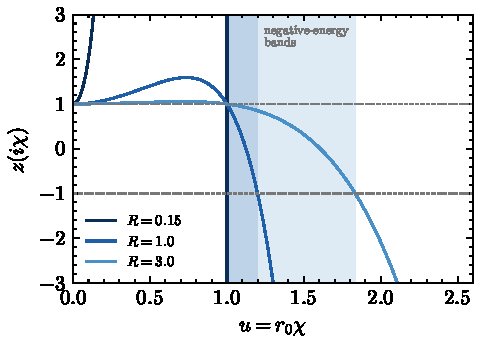
\includegraphics[width=\columnwidth]{fig_krein_band.pdf}
\caption{Half-trace $z(i\chi)$ of the transfer matrix of one period (one positive and one negative row) of the matched alternating strip, from Eq.~\eqref{eq:zchi}, plotted against the normalized decay constant $u=r_0\chi$ for loading ratios $R=r_0/a=0.15$, 1, and 3. Bloch solutions require $|z|\le1$, the region between the dashed lines. The shaded intervals $1\le u\le r_0\chi_*$, one per curve, are the negative-energy bands. Each band starts at the zone center ($z=1$) at $u=1$ and ends at the zone edge ($z=-1$) at $u=r_0\chi_*$, which defines the threshold $\chi_*$. For $R=0.15$ the band is a sliver at $u=1$, the single-row limit, too narrow to see; as $R$ grows the band widens and $\chi_*$ decreases.}
\label{fig:band}
\end{figure}

Now let the loading alternate, $r_n=(-1)^nr_0$, so that positive (ordinary) rows are interleaved with negative (non-Foster) rows and the unit cell doubles to length $2a$. The transfer matrix of the doubled cell, $T_{\rm cell}=T(-r_0)\,T(r_0)$, has half-trace
\begin{equation}
z(\kappa)=\tfrac12\operatorname{Tr}T_{\rm cell}=\cos(2\kappa a)+(r_0\kappa)^2\left[\cos(2\kappa a)-1\right],
\label{eq:z}
\end{equation}
and the Bloch condition is $\cos(2Qa)=z$, where $Q$ is the Bloch wave number of the doubled cell and the zone edge lies at $Q=\pi/2a$. For $\kappa=i\chi$, Eq.~\eqref{eq:z} becomes
\begin{equation}
z(i\chi)=1+2\sinh^2(\chi a)\left(1-r_0^2\chi^2\right),
\label{eq:zchi}
\end{equation}
and Bloch solutions with $|z|\le1$ exist only for $1/r_0\le\chi\le\chi_*$ (Fig.~\ref{fig:band}), where $\chi_*$ is the root of
\begin{equation}
\left(r_0^2\chi_*^2-1\right)\sinh^2(\chi_*a)=1 .
\label{eq:chistar}
\end{equation}
The band starts at the zone center ($z=1$) at $\chi=1/r_0$ and ends at the zone edge ($z=-1$) at $\chi=\chi_*$. It is the only band with $\kappa^2<0$, so it contains every negative-energy mode, and by Eq.~\eqref{eq:omega} all of them have real frequency if and only if
\begin{equation}
k_x\ \ge\ \chi_* .
\label{eq:threshold}
\end{equation}
Below threshold the fastest-growing mode sits at the band edge $\chi=\chi_*$, with
\begin{equation}
\sigma_{\max}=v_p\sqrt{\chi_*^2-k_x^2},\qquad \operatorname{Re}\omega=0 .
\label{eq:sigma}
\end{equation}
This mode lies at the zone edge, where the group velocity vanishes, so the instability is absolute rather than convective~\cite{Briggs_1964:book}: it grows in place. Matched terminations cannot carry it away, and shortening the strip does not remove it. A finite strip samples the band, its most strongly bound mode approaches $\chi_*$ from below as the strip grows, and the infinite-strip criterion~\eqref{eq:threshold} is therefore slightly conservative (Appendix~\ref{app:numerics}).

\begin{figure}[t]
\centering
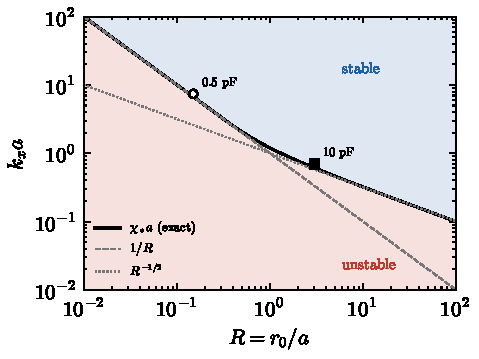
\includegraphics[width=\columnwidth]{fig_phase.pdf}
\caption{Stability diagram of the matched alternating strip in the plane of loading ratio $R=r_0/a$ and normalized transverse wave number $k_xa$. The strip is stable (blue) above the solid line $k_x=\chi_*$, computed exactly from Eq.~\eqref{eq:chistar}, and grows without oscillation (red) below it. The dashed and dotted lines are the weak- and strong-loading limits $\chi_*a\simeq1/R$ and $\chi_*a\simeq R^{-1/2}$. Grounded edges set $k_x=\pi/W_x$. The open circle marks a 0.5-pF design ($R=0.15$, $W_x=4.72$~mm, 10\% narrower than the widest stable strip of 5.24~mm), whose instability scale is 12.7~GHz. The filled square marks the 10-pF design of Sec.~\ref{sec:hardware} ($R=3.0$, $W_x=50$~mm, 12\% narrower than the 57.1-mm limit), whose instability scale is 1.17~GHz. Losses are not included; with losses the blue region carries loss-driven oscillation unless the NICs supply gain (Sec.~\ref{sec:loss}).}
\label{fig:phase}
\end{figure}

The threshold has simple limits. For weak loading, $r_0\ll a$, the band is a sliver above $1/r_0$ and
\begin{equation}
\chi_*\simeq\frac{1}{r_0}\left(1+2e^{-2a/r_0}\right),
\label{eq:weak}
\end{equation}
while for strong loading, $r_0\gg a$,
\begin{equation}
\chi_*\simeq\frac{1}{\sqrt{r_0a}} .
\label{eq:strong}
\end{equation}
Between these limits $\chi_*$ decreases monotonically with $r_0$ (Fig.~\ref{fig:phase}), so stronger negative loading is more stable. A larger $|C_L|$ binds its negative-energy mode less tightly, with a decay length of order $r_0$, and less transverse confinement is then needed to lift the mode above dc. This runs against the intuition that a stronger active element is more dangerous. It is a statement about ideal elements, however, and Sec.~\ref{sec:hardware} discusses what it costs in hardware. With grounded edges, $k_x=\pi/W_x$, and Eq.~\eqref{eq:threshold} becomes the width rule
\begin{equation}
W_x\ \le\ \frac{\pi}{\chi_*(r_0/a)} .
\label{eq:width}
\end{equation}
Grounding is a structural requirement rather than a convenience. An open (magnetic-wall) edge readmits $k_x=0$, which lies below threshold for every $r_0$, and the strip then grows at the rate $v_p\chi_*$.

\section{Role of the series inductance}
\label{sec:series}

\begin{figure*}[t]
\centering
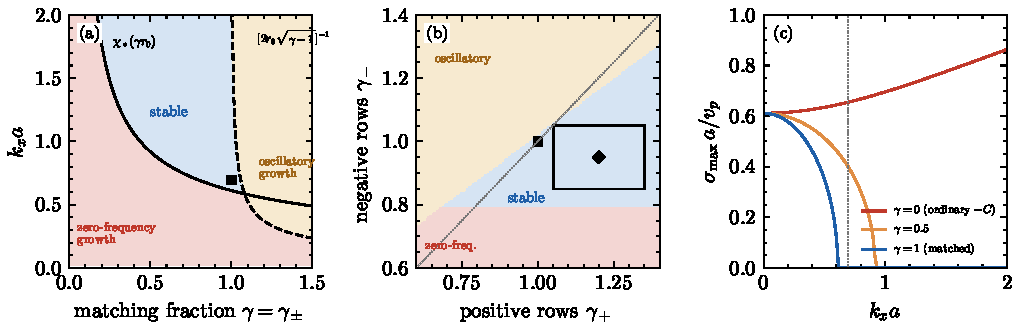
\includegraphics[width=\textwidth]{fig_matching.pdf}
\caption{Tolerance to imperfect matching between shunt and series elements on the infinite lossless strip, computed with the exact transfer matrix. Blue regions are stable, red regions grow without oscillation (real pole), and ochre regions grow with oscillation (complex pole pair). (a) Both row types carry the same fraction $\gamma$ of the matched series admittance, at $R=3$. The solid line is the under-matching threshold $k_x=\chi_*(\gamma r_0)$, the dashed line is the over-matching limit $k_x=[2r_0\sqrt{\gamma-1}]^{-1}$, and the square marks the 10-pF design at $\gamma=1$, $k_xa=0.70$. (b) Separate fractions $\gamma_+$ and $\gamma_-$ on the positive and negative rows at the design point ($R=3.0$, $k_xa=0.70$). Nominal matching (square) lies on the edge of the stable wedge. The biased design $(\gamma_+,\gamma_-)=(1.2,0.95)$ (diamond) sits inside it, and the rectangle around the diamond, with half-widths $0.15$ in $\gamma_+$ and $0.10$ in $\gamma_-$, is stable throughout. The dotted diagonal is $\gamma_+=\gamma_-$. (c) Largest growth rate $\sigma_{\max}$, in units of $v_p/a$, versus $k_xa$ for $R=3$ and $\gamma=0$ (ordinary negative capacitors without series elements), $0.5$, and $1$ (matched). Without series elements the growth increases as the strip narrows, whereas matched loading is stabilized at $k_x=\chi_*$. The dotted vertical line marks the design width $W_x=50$~mm.}
\label{fig:matching}
\end{figure*}

The matched pair $(\pm C_L,\pm L_L)$ is what makes a threshold exist. To see this, let each row carry only a fraction $\gamma_n$ of the matched series admittance, $L_L\to L_L/\gamma_n$. Equation~\eqref{eq:gevp} then generalizes to
\begin{equation}
-\phi''+k_x^2W_\gamma\,\phi=\frac{\omega^2}{v_p^2}\,W\phi,\qquad
W_\gamma=1+2\sum_n\gamma_nr_n\delta(y-na),
\label{eq:gamma}
\end{equation}
in which $\gamma_n=1$ is matched loading and $\gamma_n=0$ describes ordinary shunt capacitors without series elements.

For ordinary negative capacitors, $\gamma_n=0$, the left side of Eq.~\eqref{eq:gamma} is a positive operator for every $k_x$, namely the inductive energy of the host alone. More generally, the modes of any lossless network of positive inductors solve $K\bm u=\omega^2C\bm u$, where $K$ is the positive-definite inductive Laplacian and $C$ the nodal capacitance matrix. By Sylvester's law of inertia~\cite{Horn_2013:book} the number of modes with $\omega^2<0$ equals the number of negative eigenvalues of $C$ (Appendix~\ref{app:inertia}). The rule that the total capacitance must be positive is the one-node case of this statement and is correct only when the positive and negative capacitors share a node. A positive and a negative capacitor at different nodes give an indefinite $C$ and are unstable for any length of the connecting line, as found in Ref.~\cite{Loncar_2017:TAP}. No choice of width, length, or termination changes the inertia of $C$, and narrowing the strip in fact makes matters worse: an isolated ordinary negative row has
\begin{equation}
\sigma^2=\frac{v_p^2}{2r_0^2}\left[1+\sqrt{1+4r_0^2k_x^2}\right],
\label{eq:sigma0}
\end{equation}
which grows with $k_x$ [Fig.~\ref{fig:matching}(c)]. A negative capacitor leaves the transverse inductive stiffness untouched, so confinement cannot restore what the capacitor removes.

With a common fraction $0<\gamma\le1$ on all rows, the zero-frequency band edge follows from Eq.~\eqref{eq:chistar} with $r_0\to\gamma r_0$. The strip is stable if and only if
\begin{equation}
k_x\ \ge\ \chi_*(\gamma r_0),
\label{eq:undermatch}
\end{equation}
and no oscillatory modes appear. Under-matching thus costs width, and the threshold diverges as $\gamma\to0$. Over-matching, $\gamma>1$, introduces a second kind of failure. Each negative row then binds, besides its negative-energy mode, a positive-energy mode below the transverse cutoff. The two are the roots of
\begin{equation}
r_0^2\left(\gamma k_x^2-x\right)^2=k_x^2-x,\qquad x=\omega^2/v_p^2 ,
\label{eq:quad}
\end{equation}
which are the band edges $q^2=1$ of the exact half-trace (Appendix~\ref{app:gamma}), and they collide at finite frequency when the discriminant of Eq.~\eqref{eq:quad} changes sign. Stability then requires
\begin{equation}
4r_0^2k_x^2(\gamma-1)\ \le\ 1 ,
\label{eq:overmatch}
\end{equation}
and beyond this limit the strip oscillates at $\omega\simeq v_p(k_x^2-1/4r_0^2)^{1/2}$, just below the transverse cutoff. This is a Krein collision at nonzero frequency, a complex pole pair in circuit language. Condition~\eqref{eq:overmatch} does not depend on the row spacing. Together, Eqs.~\eqref{eq:undermatch} and~\eqref{eq:overmatch} give the stability window
\begin{equation}
\chi_*(\gamma r_0)\ \le\ k_x\ \le\ \frac{1}{2r_0\sqrt{\gamma-1}}
\label{eq:window}
\end{equation}
shown in Fig.~\ref{fig:matching}(a).

Matching errors on the positive and negative rows act differently [Fig.~\ref{fig:matching}(b)]. The governing rule is that no row may bind a positive-energy mode below the transverse cutoff. Such a mode appears whenever a negative row is over-matched ($\gamma_->1$) or a positive row is under-matched ($\gamma_+<1$), and once it hybridizes with the negative-energy band the pair leaves the real axis and the strip oscillates. Nominal matching therefore sits on the edge of the stable region. At the design point of Sec.~\ref{sec:hardware}, independent errors of $\pm0.5\%$ in $\gamma_\pm$ are tolerated, but $\pm1\%$ already reaches the oscillatory region when $\gamma_+$ errs low while $\gamma_-$ errs high. The tolerance widens considerably when the matching is deliberately biased, with the passive rows over-matched and the active rows under-matched. For $(\gamma_+,\gamma_-)=(1.2,0.95)$ the strip remains stable for independent deviations of $\pm0.15$ in $\gamma_+$ and $\pm0.10$ in $\gamma_-$. Expressed through the series inductors themselves, which scale as $1/\gamma$, the biased design tolerates independent errors of $\pm12\%$ in the passive inductors and $\pm10\%$ in the NIC inductors.

\section{Design example}
\label{sec:hardware}

\begin{table}[t]
\caption{Design values for a host with $C'=150$~pF/m and $Z_0=50~\Omega$ ($v_p=1.33\times10^8$~m/s, $L'=375$~nH/m), row spacing $a=11.1$~mm, and lane pitch $\Delta_x=5$~mm. The instability scale is $\nu_*=v_p\chi_*/2\pi$, and $W_{x,\max}=\pi/\chi_*$ is the widest stable grounded strip.}
\label{tab:hardware}
\begin{ruledtabular}
\begin{tabular}{cccccc}
$C_L$ (pF) & $r_0$ (mm) & $r_0/a$ & $\chi_*$ (m$^{-1}$) & $\nu_*$ (GHz) & $W_{x,\max}$ (mm) \\ \hline
0.5 & 1.67 & 0.15 & 600.0 & 12.73 & 5.24 \\
2   & 6.67 & 0.60 & 159.1 & 3.37 & 19.8 \\
5   & 16.7 & 1.50 & 82.7 & 1.76 & 38.0 \\
10  & 33.3 & 3.00 & 55.1 & 1.17 & 57.1 \\
20  & 66.7 & 6.01 & 37.8 & 0.80 & 83.1 \\
50  & 167  & 15.0 & 23.5 & 0.50 & 133.6 \\
\end{tabular}
\end{ruledtabular}
\end{table}

We take a 50-$\Omega$ host with $C'=150$~pF/m, which gives $v_p=1/(Z_0C')\approx1.33\times10^8$~m/s $\approx c/2.25$, typical of a printed line on a moderate-permittivity substrate~\cite{Pozar_2012:book}. Rows are spaced by $a=11.1$~mm and the lane pitch is $\Delta_x=5$~mm, so that $C_0=0.75$~pF and $L_0=1.875$~nH. Table~\ref{tab:hardware} lists the resulting threshold for several load values.

The threshold is the boundary for ideal, lossless, dispersionless elements, and what the hardware must supply is set by where the negative-energy modes live. The elements must present their nominal negative values for complex frequencies up to $|s|\sim v_p\chi_*$, which in practice means up to the transverse cutoff $\nu_c=v_pk_x/2\pi\ge\nu_*$. Table~\ref{tab:hardware} shows that this scale is set by $C_L$: a 0.5-pF load places it at 12.7~GHz, whereas large loads bring it into the low-gigahertz range. The same condition explains why stable one-dimensional non-Foster lines are possible in practice~\cite{Long_2014:TMTT,Long_2018:TMTT}. A band-limited negative capacitor that stops being negative well below $|s|\sim v_p/r_0$ lies outside the ideal statement, as shown in Ref.~\cite{Loncar_2017:TAP} for the two-capacitor network.

We choose $C_L=10$~pF, for which $r_0=33.3$~mm, $r_0/a=3.0$, $\chi_*=55.1$~m$^{-1}$, and $W_{x,\max}=57.1$~mm. A strip of width $W_x=50$~mm has $k_x=62.8$~m$^{-1}$, a margin of 14\% above threshold, and a transverse cutoff at 1.33~GHz. Its negative-energy modes are stable in the lossless model and occupy the band from 0.64 to 1.17~GHz, which is the range over which the NICs must be accurate. The matched series inductance is $L_L=0.141$~nH per link, and the discrete-row correction to $k_x$ is $-0.4\%$. With a uniform matching error, Eqs.~\eqref{eq:undermatch} and~\eqref{eq:overmatch} allow $0.79\le\gamma\le1.057$. With the biased design $(\gamma_+,\gamma_-)=(1.2,0.95)$, the series elements are $0.117$~nH on positive rows and $-0.148$~nH on negative rows, and each negative row requires 9 shunt and 10 series non-Foster elements. The internal stability of each NIC is a separate circuit-level requirement that the lattice model does not address~\cite{Suarez_2018:TMTT}.

This design is demanding, and the demand comes from the matched pair. Because $L_LC_L=(\Delta_x/v_p)^2$, a $-10$-pF shunt capacitor must be paired with a series inductance of about $-0.15$~nH, smaller than the parasitic inductance of a typical surface-mount component, and the 19 NICs of each negative row must hold their values to about $\pm10\%$ up to 1.3~GHz. That is beyond the non-Foster elements demonstrated so far; for comparison, the negative capacitor of Ref.~\cite{Long_2014:TMTT} realizes $-10$~pF over 10--150~MHz. The design scales, however. Multiplying all lengths and $C_L$ by a factor $s$ at fixed host leaves $R$, $k_xa$, and every dimensionless result unchanged, divides all frequencies by $s$, and multiplies $L_L$ by $s$. For $s=8$ the negative-energy band moves to 80--146~MHz and the cutoff to 167~MHz, with $C_L=80$~pF, $L_L=1.1$~nH, $a=89$~mm, $\Delta_x=40$~mm, and a strip 40~cm wide. The same scaling shows the cost of the result that stronger negative loading is more stable. A larger $C_L$ lowers the instability scale, but at fixed lane pitch it requires a proportionally smaller matched series inductance, so the advantage holds for ideal elements and must be weighed against what the NIC can realize.

The design suggests bench tests that need no circuit-level pole identification. At a fixed width of 50~mm, increasing the magnitude of the loads should switch the strip from exponential runaway without a carrier, $\operatorname{Re}\omega=0$, to the regime above threshold at $C_L=7.92$~pF, so that latch-up disappears on the side of stronger negative loading. Below threshold the envelope should grow as $e^{\sigma_{\max}t}$, following Eq.~\eqref{eq:sigma}, and sweeping $W_x$ at fixed $C_L$ while fitting $\sigma_{\max}^2$ against $k_x^2$ measures $\chi_*$ directly. Above threshold a strip without gain compensation should oscillate inside the negative-energy band at a rate set by the loss (Sec.~\ref{sec:loss}), a signature that distinguishes the two regimes by the presence of a carrier. Detuning the series elements uniformly should produce latch-up below $\gamma\approx0.79$ and oscillation near 1.29~GHz above $\gamma\approx1.057$, while removing them altogether ($\gamma=0$) should destabilize the strip at every width, with faster growth for narrower strips. Replacing the grounded edges by open ones readmits $k_x=0$ and should give runaway at $\sigma=v_p\chi_*=7.3\times10^{9}$~s$^{-1}$ at any width.

\section{Effect of loss}
\label{sec:loss}

Above threshold the strip still carries negative-energy modes at real frequency, between 0.64 and 1.17~GHz in the design above, and for such modes dissipation is destabilizing~\cite{Cairns_1979:JFM,MacKay_1991:PLA,Kirillov_2013:book}. The mechanism follows from energy balance. Give every element $e$ a small loss tangent $d_e=1/Q_e$, with $d_e>0$ for dissipation, so that a mode with time-averaged element energies $U_e$ (signed, with $U=\sum_eU_e$) dissipates the power $P=2\omega\sum_e|U_e|\,d_e$. Since $dU/dt=-P$, the mode amplitude changes at the rate
\begin{equation}
\sigma=-\frac{\omega}{U}\sum_e|U_e|\,d_e .
\label{eq:losssigma}
\end{equation}
Positive-energy modes decay, as in any passive structure, but a negative-energy mode, $U<0$, grows: losing energy makes its total energy more negative and its amplitude larger. With a uniform quality factor $Q$, Eq.~\eqref{eq:losssigma} becomes $\sigma=\Lambda\,\omega/Q$, where $\Lambda=\sum_e|U_e|/|U|\ge1$. The participation ratio $\Lambda$ exceeds one because the net energy of a negative-energy mode is the difference between the positive energy stored in the host and the passive rows and the larger negative energy stored on the NIC rows. For the 10-pF design, the finite-strip eigenvectors of Appendix~\ref{app:numerics} give $\Lambda=3.6$--$7.8$ across the band of the lowest transverse order. For $Q=100$, a direct solution of the lossy eigenproblem, without perturbation theory, gives a largest growth rate of $4.6\times10^8$~s$^{-1}$ at 1.14~GHz, an $e$-folding time of 2.2~ns, in agreement with Eq.~\eqref{eq:losssigma}. Resistive terminations act in the same way, since inside the band the negative-energy modes propagate and a resistive load drains energy from them.

Loss therefore leaves the location of the threshold unchanged but alters its meaning. Below $k_x=\chi_*$ the strip latches up at the ideal rate~\eqref{eq:sigma}, and above it a lossy strip oscillates inside the negative-energy band at a rate proportional to the loss, which for $Q\approx100$ is more than an order of magnitude slower than the open-edge latch-up rate.

The remedy is gain on the active rows. An NIC presents the negative of its load impedance~\cite{Linvill_1953:PIRE}, so a negative capacitor synthesized from a lossy capacitor carries a negative series resistance and acts as an element with $d_e<0$. Negative-energy modes are concentrated on the NIC rows, whereas positive-energy modes reside mostly in the host and the passive rows, so the two kinds of mode weight the NIC gain differently in Eq.~\eqref{eq:losssigma}. Let all passive elements have loss tangent $d$ and all NIC elements $-\rho d$, and split $\Lambda=\Lambda_P+\Lambda_N$ into its passive and NIC shares. Every negative-energy mode then decays when $\rho$ exceeds the largest ratio $\Lambda_P/\Lambda_N$ among the negative-energy modes, and every positive-energy mode decays when $\rho$ is below the smallest such ratio among the positive-energy modes. For the 10-pF design this window is $0.77<\rho<1.37$. The lowest transverse order sets it, and the higher orders checked, up to $m=6$, give slightly wider windows. The direct lossy solution agrees: at $Q=100$ the strip still grows for $\rho=0.7$, is stable from $\rho=0.8$ to $1.35$, and for $\rho=1.4$ a positive-energy mode near 1.34~GHz becomes unstable. Full stability thus requires a net NIC gain that balances the passive loss to within about $\pm30\%$, a requirement of the same kind as the matching tolerance of Sec.~\ref{sec:series}. This estimate treats each loss as a frequency-independent loss tangent; in a real NIC the gain is dispersive and has to satisfy the window across the negative-energy band and the positive-energy modes just above it.

\section{Discussion and conclusion}
\label{sec:discussion}

The energy metric gives a common account of the difficulties set out in Ref.~\cite{Hrabar_2018:EPJAM}. That review stresses that methods based on the input impedance or reflection coefficient of a single port fail because of hidden modes, and that only methods taking all meshes and nodes of the network into account can be trusted. In the present picture the hidden modes are the negative-energy modes. The instability is a property of the capacitance metric $W(y)$ inside the structure: the threshold~\eqref{eq:threshold} depends only on $r_0$, $a$, and $k_x$, none of which is a port quantity, and whether a negative-energy mode is visible at a port depends on how strongly the port couples to it, which is precisely the information a port reduction discards. Because the mode is absolute, it also does not need to reach a port in order to grow. The inertia count is an all-node criterion of the kind the review calls for. It replaces the rule that the overall mesh capacitance must be positive, to which it reduces when the positive and negative capacitors share a node, and it accounts for the two exceptions to that rule that the review describes. A network built entirely from negative elements is stable, because reversing the signs of both $K$ and $C$ leaves the pencil $K\bm u=\omega^2C\bm u$ unchanged (Appendix~\ref{app:inertia}); every mode then carries negative energy, and modes that all carry the same energy sign cannot undergo a Krein collision. Negative elements without positive swamping elements next to them, as in the equivalent circuit of an ideal transformer, are harmless as long as the full inductance matrix stays positive definite, as it does for any physical pair of coupled coils, because stability is decided by the inertia of the full matrices and not by the sign of any single element. The velocity-matched rows are a distributed example: each negative capacitor is accompanied by a negative series inductance, and stability is decided by $k_x$ against $\chi_*$ rather than by any condition on total reactance.

The review also emphasizes that a realistic negative element is band-limited and always accompanied by an unwanted resistance, positive or negative. Band limitation enters through the validity condition of Sec.~\ref{sec:hardware}, and the review suggests it as the reason why early one-dimensional lines worked even though ideal-element analyses predicted instability. The sign of the resistance is decisive, as Sec.~\ref{sec:loss} shows. Positive resistance drives the negative-energy modes unstable, whereas negative resistance inside the window $0.77<\rho<1.37$ damps them without destabilizing the positive-energy modes. This is the distributed counterpart of the lumped circuits of Ref.~\cite{Hrabar_2018:EPJAM}, in which a positive part joined to an all-negative part is stable when the overall resistance, capacitance, and inductance are negative: a mode of negative energy needs negative resistance to decay. The review closes by calling for a framework that connects causality, stability, and nonlinearity. For linear networks the energy signature supplies the stability part of such a framework, and its extension to loss and gain is where it meets causality, since a band-limited negative element is necessarily lossy or active.

The length dependence follows as well. A finite matched strip has one negative-energy mode per negative row, and as the strip grows these modes fill the band and the most strongly bound one approaches $\chi_*$. Stability of a short section therefore does not guarantee stability of a long one, consistent with Ref.~\cite{Rengarajan_2013:AWPL}, and the infinite-strip criterion is the length-independent bound.

The analysis leaves out several features of real hardware. The model is continuous along the stacking direction and treats the lumped character of the rows only through the exact discrete-row correction, and it has not been checked against a circuit simulation of the lumped network with realistic NIC models. NIC dispersion and nonlinear saturation~\cite{Okorn_2017:Automatika} shift the ideal threshold, and the loss analysis of Sec.~\ref{sec:loss} is first order in the loss and assumes frequency-independent quality factors. Each of these extensions can be treated as a perturbation of the exact Krein structure presented here, and the loss-gain window is the first such perturbation that a realistic design has to satisfy.

Loading a transmission-line medium with shunt capacitors changes its energy metric rather than its stiffness, and this single observation turns non-Foster stability into a kinematic question with closed-form answers. Ordinary negative capacitors are unstable whenever the capacitance matrix is indefinite, regardless of geometry. Velocity-matched negative loading is free of latch-up when transverse confinement exceeds the binding of the negative-energy band, $k_x\ge\chi_*$, imperfect matching opens an asymmetric tolerance window that can be designed, and the loss that would destabilize the surviving negative-energy modes can be balanced by a controlled NIC gain. The resulting rules are geometric, $W_x\le\pi/\chi_*$, and they place the instability scale where the NICs must operate.

\begin{acknowledgments}
D.~\v{S}$^1$. and D.~S. are partially supported by the US National Science Foundation, under Grant No.~PHY-2310363. Claude Opus 5.5 was used in assisting with text and numerical code, as well as auditing earlier versions of the manuscript. 
\end{acknowledgments}

\bibliography{references}

\appendix

\section{Inertia and reality of the spectrum}
\label{app:inertia}

Consider a lossless network with node fluxes $\bm\Phi$, so that the node voltages are $\dot{\bm\Phi}$, a nodal capacitance matrix $C$ that is real, symmetric, and possibly indefinite, and an inductive Laplacian $K$. Nodes connected only through capacitors are first eliminated by Kron reduction of $C$, so that $K$ is positive definite once the network is grounded. The equations of motion $C\ddot{\bm\Phi}=-K\bm\Phi$ give modes $K\bm u=\omega^2C\bm u$, and with $\bm u=K^{-1/2}\bm v$ this becomes
\begin{equation}
K^{-1/2}CK^{-1/2}\,\bm v=\omega^{-2}\,\bm v,
\end{equation}
a real symmetric eigenproblem, so $\omega^2$ is real. The matrix $K^{-1/2}CK^{-1/2}$ is congruent to $C$, and by Sylvester's law of inertia~\cite{Horn_2013:book} it has as many negative eigenvalues as $C$. Each of them gives $\omega^2<0$, that is, a real right-half-plane pole, which proves the inertia count used in Sec.~\ref{sec:series}. The same argument holds when $K$ is negative definite, as in a network built entirely from negative inductors, with $-K$ in place of $K$; the number of modes with $\omega^2<0$ is then the number of positive eigenvalues of $C$. Whenever $K$ is definite, it is therefore the inertia of $C$ relative to $K$, and not the sign of any element, that decides stability, and a lossless network whose elements are all negative is as stable as one whose elements are all positive. For matched loading, $K$ and $C$ share the row structure, and the problem separates into transverse orders. For each order the same argument applies to the pair $(-\partial_y^2,W)$ with eigenvalue $\kappa^2$, so the eigenvalues $\kappa^2$ are real and the number with $\kappa^2<0$ equals the number of negative rows. The transverse term then shifts every $\omega^2$ by $v_p^2k_x^2$, which is how confinement lifts the negative-energy modes.

\section{Transfer matrix with general matching}
\label{app:gamma}

Between rows, solutions of Eq.~\eqref{eq:gamma} vary as $e^{\pm\mu y}$ with $\mu^2=k_x^2-x$ and $x=\omega^2/v_p^2$. A row of strength $r$ and matching fraction $\gamma$ imposes the jump $\phi'(na^+)-\phi'(na^-)=g\,\phi(na)$ with $g=2r(\gamma k_x^2-x)$. For rows with jumps $g_1$ and $g_2$ alternating at spacing $a$, the half-trace of the doubled cell is
\begin{equation}
z=\cosh(2\mu a)+\frac{g_1+g_2}{2\mu}\sinh(2\mu a)+\frac{g_1g_2}{2\mu^2}\sinh^2(\mu a),
\end{equation}
which for equal and opposite jumps, $g_{1,2}=\pm g$, reduces to
\begin{equation}
z=1+2\sinh^2(\mu a)\,(1-q^2),\qquad q=\frac{r_0(\gamma k_x^2-x)}{\mu},
\end{equation}
and for $\gamma=1$ and $\mu=\chi$ reproduces Eq.~\eqref{eq:zchi}. The zero-frequency boundary is $z(x=0)=-1$, which is Eq.~\eqref{eq:chistar} with $r_0\to\gamma r_0$. For $\gamma\le1$ we verified numerically, but have not proved, that $z$ decreases monotonically along $x<0$, so that this boundary is the full zero-frequency criterion.

The points $q^2=1$ are where $z=1$ for any $a$. They are the roots of the quadratic~\eqref{eq:quad}, whose discriminant is $D=1+4r_0^2k_x^2(1-\gamma)$. For $\gamma\le1$, $D>0$ and only one root lies on the physical sheet. For $\gamma>1$ both roots are physical bound modes, of opposite energy sign. They merge at $D=0$, beyond which the maximum of $z$ between them falls below one and a complex-conjugate pair of $x$ appears. This gives Eq.~\eqref{eq:overmatch}, with the merging point at $x=k_x^2-1/4r_0^2$.

\section{Numerical checks}
\label{app:numerics}

The closed-form statements were compared with a finite-difference solution of Eq.~\eqref{eq:gamma} on finite strips with Dirichlet ends, solved as a general generalized eigenproblem without using the transfer matrix, so that complex eigenvalues are not excluded by construction. Both methods solve the same continuum model, so the comparison tests the algebra and the closed forms, not the model itself. For $R=0.15$ and $R=3$ with 10 negative rows the solver finds exactly 10 negative-energy modes. For $R=3$ they lie at $\chi a\in[0.360,0.611]$, inside the band $[1/R,\chi_*a]=[0.333,0.611]$, and finite strips of 10, 20, and 40 rows approach $\sigma_{\max}$ of Eq.~\eqref{eq:sigma} from below. For $\gamma=1$, 0.75, 0.5, and 0.25 the strip is unstable at $k_x=0.99\,\chi_*(\gamma r_0)$ and stable at $1.01\,\chi_*(\gamma r_0)$, with no complex eigenvalues. For $\gamma=0$ every transverse wave number tested is unstable with one growing mode per negative row, and the isolated-row rate~\eqref{eq:sigma0} is reproduced to better than 0.1\%. The over-matching onset~\eqref{eq:overmatch} agrees with the lattice computation to $10^{-10}$, and the two colliding modes carry opposite energy signs. The tolerance map of Fig.~\ref{fig:matching}(b) was computed from the exact half-trace and spot-checked by finite differences at the corners and center of the biased tolerance rectangle. The loss results of Sec.~\ref{sec:loss} use the same finite strip with 40 rows: the participation ratios come from its lossless eigenvectors, and the growth rates from the complex generalized eigenproblem in which each element value $X_e$ is replaced by $X_e+i|X_e|d_e$. Near each boundary finite strips are slightly more stable than the infinite strip, so the numbers quoted in the paper are infinite-strip values unless stated otherwise. The scripts that reproduce every number and figure are provided as Supplemental Material.

\end{document}
